% !TEX program = pdflatex
\documentclass[conference]{IEEEtran}
\IEEEoverridecommandlockouts

\usepackage{cite}
\usepackage{amsmath,amssymb,amsfonts}
\usepackage{algorithm}
\usepackage{algorithmic}
\usepackage{graphicx}
\usepackage{textcomp}
\usepackage{xcolor}
\usepackage{tikz}
\usetikzlibrary{arrows,positioning,calc,shapes.geometric,fit,arrows.meta}
\usepackage{booktabs}
\usepackage{array}
\usepackage{listings}
\lstset{
  language=Java,
  basicstyle=\ttfamily\tiny,
  breaklines=true,
  frame=single,
  numbers=left,
  numberstyle=\tiny,
  numbersep=3pt,
  xleftmargin=6pt,
  framexleftmargin=6pt,
}

\def\BibTeX{{\rm B\kern-.05em{\sc i\kern-.025em b}\kern-.08em
    T\kern-.1667em\lower.7ex\hbox{E}\kern-.125emX}}

\begin{document}

\title{Dependency-Aware Code Smell Refactoring\\via Multi-Agent LLM System}

\author{
\IEEEauthorblockN{Havriil Pietukhin, Ivan Polasek}
\IEEEauthorblockA{
  \textit{Department of Applied Informatics}\\
  \textit{Comenius University in Bratislava}\\
  Bratislava, Slovakia\\
  pietukhin1@uniba.sk}
}

\maketitle

\begin{abstract}
This paper proposes a multi-agent system combining SonarQube-based code smell
detection with a dependency-aware Best-First Search planner and LLM-driven
refactoring agents to automatically improve Java code quality.
Existing LLM-based refactoring approaches treat each code smell in isolation,
ignoring causal dependencies between operations that can introduce new smells
or require additional corrective steps.
We formalize a dependency model capturing positive and negative interactions
between refactoring operations, which the Best-First Search planner exploits
to always select the most beneficial next refactoring step according to a
heuristic scoring function.
Analysis of examples from the RefactoringMiner~2.0 dataset (15,562 refactorings,
188 repositories) and SWE-Refactor (1,099 records) demonstrates that a greedy
baseline introduces up to 2 new smells and requires twice as many steps,
whereas the BFS planner consistently finds shorter, higher-quality plans.
\end{abstract}

\begin{IEEEkeywords}
code smells, refactoring, dependencies, Best-First Search,
multi-agent systems, LLM, SonarQube
\end{IEEEkeywords}

%----------------------------------------------------------------------
\section{Introduction}
%----------------------------------------------------------------------

Code smells~\cite{Fowler1999}---symptoms of poor object-oriented design---
accumulate in long-lived projects, reducing readability and increasing
maintenance cost.
More than 59\% of smell-bearing classes contain multiple co-occurring
smells~\cite{palomba2018diffuseness}, and their combination degrades
comprehension significantly beyond any single smell in
isolation~\cite{abbes2011empirical}.
Recent LLM-based tools automate individual refactorings~\cite{10.1145/3691620.3695508,liang2025smelldetector},
but treat each smell independently.

Cedrim et al.~\cite{cedrim2017} showed that 57\% of refactorings in a
longitudinal study of 23 Java projects did not reduce the smell count,
and some increased it.
The root cause is \textit{inter-smell dependency}: refactoring one smell can
resolve or introduce others depending on the order of operations and the
current state of the class.
Markovič~\&~Polášek~\cite{markovic2016refaktorovanie} formalised these
positive and negative dependency rules, but no automated system uses them to
plan refactoring sequences.
We present a six-agent pipeline that models smell dependencies as a directed
graph; the planning agent uses Best-First Search (BFS) to compute an ordering
that minimises total residual smell severity, then the LLM refactoring agent
executes each operation with test-based verification.

%----------------------------------------------------------------------
\section{Related work}
%----------------------------------------------------------------------

\subsection{Code smell detection}

The CK metrics suite~\cite{chidamber1994metrics} (WMC, CBO, LCOM, RFC)
underpins threshold-based detectors; Lanza~\&~Marinescu~\cite{lanza2006object}
systematised detection rules over these metrics, laying the foundation for
tools such as iPlasma and JDeodorant.
Fontana et al.~\cite{fontana2016comparing} showed that SVM reaches 96\%
accuracy on four smell types across 74 Java projects, with Random Forest
emerging as the most consistent classifier; graph neural network approaches
later captured structural AST dependencies, outperforming metric-based
baselines on Long Method and Blob detection.
Yamashita~\&~Moonen~\cite{yamashita2013exploring} established that co-located
smells intensify maintenance problems beyond their individual effects, and
Palomba et al.~\cite{palomba2018diffuseness} confirmed in a study of 395
releases of 30 open-source projects that 59\% of smell-bearing classes contain
more than one smell type.
Abbes et al.~\cite{abbes2011empirical} further showed that combinations of God
Class and Spaghetti Code reduce developer comprehension by 124\% compared to
either smell in isolation.

\subsection{Code refactoring}

Cedrim et al.~\cite{cedrim2017} annotated 16,566 refactorings in 23 projects
as smell-reducing, smell-introducing, or neutral, finding that 57\% of
operations did not reduce the smell count and that some increased it.
This provides the clearest empirical evidence that execution order determines
whether automated refactoring improves or worsens a codebase.
Markovič~\&~Polášek~\cite{markovic2016refaktorovanie} derived a catalogue of
positive dependencies (refactoring smell $A$ may resolve smell $B$ as a side
effect) and negative dependencies (refactoring $A$ may introduce $B$),
grounded in Fowler's refactoring catalogue~\cite{Fowler1999}.
The key observation is that negative edges are state-dependent: a negative
dependency fires only if certain structural conditions hold in the class at
the time of refactoring, meaning early removal of prerequisite smells can
suppress the negative edge entirely.
No prior automated system uses this catalogue to sequence refactoring
operations.

\subsection{Large language models for code}

CodeBERT~\cite{feng2020codebert} established pre-trained transformer
representations for programming languages; subsequent parameter-efficient
fine-tuning (LoRA) applied to models such as DeepSeek-Coder and StarCoder
achieves competitive smell detection with lower computational cost.
iSMELL~\cite{10.1145/3691620.3695508} (ASE~2024) combines a Mixture-of-Experts
architecture with static analysis toolsets, achieving F1\,=\,75.17\% on seven
smell types and improving over standalone LLMs by 35\% in F1.
SmellDetector~\cite{liang2025smelldetector} (IJCNN~2025) fine-tunes LLMs for
multi-label smell detection and identifies refactoring opportunities across
Java projects as a multi-label classification task.
Both iSMELL and SmellDetector target individual smell instances; neither
models the interaction between sequential refactoring operations or uses
dependency-aware planning to order them.

%----------------------------------------------------------------------
\section{Our Approach}
%----------------------------------------------------------------------

\subsection{Method overview}

The pipeline comprises ten agents (A--J) shown in Fig.~\ref{fig:pipeline}.
\textbf{A}~loads the source code and detects the build system (Maven or Gradle).
\textbf{B}~checks whether every function has a corresponding test.
\textbf{C}~generates any missing tests via LLM (skipped if all tests exist).
\textbf{D}~runs the full test suite to record a pre-refactoring baseline.
\textbf{F}~scans the target commit via the SonarQube REST API and normalises
the output into typed smell instances with severity labels (HIGH\,=\,3,
MEDIUM\,=\,2, LOW\,=\,1).
\textbf{G}~presents detected smells to the developer for selection.
\textbf{E}~constructs the inter-smell dependency graph (DAG).
\textbf{H}~runs Best-First Search on the DAG to produce the ordered plan~$\pi$.
\textbf{I}~executes each planned refactoring using a chain-of-thought LLM prompt.
\textbf{J}~runs the test suite after refactoring, rolls back and replans via~H
on failure, and compares before/after metrics on success.

\begin{figure*}[tb]
\centering
\includegraphics[width=\textwidth]{pipeline}
\caption{Multi-agent pipeline (A--J). Agent~H (BFS planner) highlighted in blue;
Agent~I (LLM refactoring) in orange; Agent~C (test generation) in green.
Dashed edge from J to H denotes rollback and replanning on test failure.}
\label{fig:pipeline}
\end{figure*}

Eight smell types are targeted, mapped to SonarQube rules
(Table~\ref{tab:smells}).

A complete run proceeds as follows.
Agent~A detects the build system (Maven or Gradle); Agent~B--C ensure a test suite is present.
Agent~F scans the target commit via the SonarQube REST API and maps each reported
issue to one of the eight types in Table~\ref{tab:smells}, assigning the
corresponding severity weight.
Agent~G lets the developer select target smells; Agent~E builds the dependency graph
(Section~III-B); Agent~H produces the ordered plan~$\pi$.
Agent~I retrieves the source file for the first item in $\pi$, calls the LLM with
a chain-of-thought prompt, validates the response against a typed schema,
and writes the patch.
Agent~J executes the test suite; a failing run triggers rollback and passes the
updated smell set back to Agent~H for replanning.
Steps I--J repeat until $\pi$ is exhausted or $h(S) = 0$.
All intermediate smell sets, dependency graphs, LLM responses, and CK metric
snapshots (WMC, CBO, RFC, LCOM) are logged to MLflow for reproducibility.

% fig:refactoring removed — consolidated into fig:pipeline (pipeline.mmd)

\begin{table}[tb]
\caption{Detected smell types and associated refactorings}
\label{tab:smells}
\centering
\footnotesize
\setlength{\tabcolsep}{3.5pt}
\begin{tabular}{@{}llll@{}}
\toprule
\textbf{Smell} & \textbf{SQ rule} & \textbf{Sev.} & \textbf{Refactoring} \\
\midrule
Long Method          & S138  & HIGH   & \textbf{Extract Method} \\
Complex Method       & S1541 & HIGH   & \textbf{Extract Method} \\
God Class            & S1200 & HIGH   & \textbf{Extract/Move} \\
Large Class          & S110  & HIGH   & \textbf{Extract Class} \\
Cond.\ Complexity    & S1067 & MEDIUM & \textbf{Extract Method} \\
Long Param.\ List    & S107  & MEDIUM & Intro.\ Param.\ Obj. \\
Dup.\ Conditions     & S1871 & MEDIUM & Consol.\ Conditional \\
Print Statements     & S106  & LOW    & Replace w.\ Logger \\
\bottomrule
\end{tabular}
\end{table}

\subsection{Smell dependency model}

Dependencies between smells are represented as a directed graph $G=(V,E)$,
where each node $s_i \in V$ is a detected smell instance.
Two edge types are defined:
\begin{itemize}
  \item \textit{positive} $s_i \xrightarrow{+} s_j$: refactoring $s_i$
        may resolve $s_j$ as a side effect;
  \item \textit{negative} $s_i \xrightarrow{-} s_j$: refactoring $s_i$
        may introduce $s_j$.
\end{itemize}
An edge is added when the smell-type pair matches a rule from the
catalogue~\cite{markovic2016refaktorovanie} and both smells reside in the same
class context.
Negative edges are state-dependent: Extract Class introduces a Long Method
only if long methods already exist in the source class---a condition that can
be avoided by refactoring Long Method first.
Table~\ref{tab:deps} lists the key rules implemented.

\begin{table}[tb]
\caption{Implemented dependency rules~\cite{markovic2016refaktorovanie}}
\label{tab:deps}
\centering
\footnotesize
\setlength{\tabcolsep}{2.5pt}
\begin{tabular}{@{}p{2.0cm}p{2.6cm}p{2.6cm}@{}}
\toprule
\textbf{Smell} & \textbf{Positive (resolves)} &
  \textbf{Negative (introduces)} \\
\midrule
Long Method / Complex &
  Feature Envy, Dup.\ Code, Long Param.\ List &
  Long Method, Long Param.\ List \\
Long Param.\ List &
  Data Clumps &
  Data Class \\
God Class / Large Class &
  Feature Envy, Data Clumps &
  Long Method, Data Class, Inapp.\ Intimacy \\
Dup.\ Conditions &
  Divergent Change &
  Large Class \\
\bottomrule
\end{tabular}
\end{table}

Fig.~\ref{fig:depgraph} visualises the full dependency graph over the eight
detected smell types.
Solid green arrows denote positive dependencies; dashed red arrows denote
negative dependencies.
Node shading indicates dataset coverage: dark nodes have ground-truth
refactoring examples in RefactoringMiner~2.0 or SWE-Refactor;
light nodes lack direct ground truth.

\begin{figure*}[tb]
\centering
\includegraphics[width=\textwidth]{depgraph}
\caption{Smell dependency tree (positive resolution edges). Blue nodes have
  ground-truth refactoring examples (\checkmark); grey nodes lack direct ground
  truth ($\times$). Dashed edge = negative dependency (may introduce).
  Severity: H\,=\,HIGH, M\,=\,MED, L\,=\,LOW.}
\label{fig:depgraph}
\end{figure*}

\subsection{Planning agent}

The general priority score for a smell $s_i$ is:
\begin{equation}
  PD_i = w \cdot \mathrm{sev}(s_i) \cdot \mathrm{freq}(s_i)
         + \textstyle\sum \mathrm{pos\_out}(s_i)
         - \textstyle\sum \mathrm{neg\_out}(s_i),
  \label{eq:pd-general}
\end{equation}
where $w$ is a weight constant (default $w{=}0.5$), $\mathrm{freq}(s_i)$ is
the occurrence count of the smell in the class, $\mathrm{pos\_out}$ counts
outgoing positive edges in the current graph, and $\mathrm{neg\_out}$ counts
outgoing negative edges.
In the concrete implementation, positive edges are counted from
smell instances actually co-located in the source, while negative edges use
the abstract catalogue rules of Markovič~\&~Polášek:
\begin{equation}
  PD^{\mathrm{conc}}_i = w \cdot \mathrm{sev}(s_i)
         + \textstyle\sum \mathrm{pos\_out}^{\mathrm{conc}}(s_i)
         - \textstyle\sum \mathrm{neg\_out}^{\mathrm{abs}}(s_i).
  \label{eq:pd-concrete}
\end{equation}
Note that positive dependencies observed in source may not materialise in
every case; empirical validation (e.g.\ from Cedrim et al.~\cite{cedrim2017})
would allow weighting each edge by its empirical probability.
Negative edges are treated as more reliable because they capture structural
risks that the planner must avoid regardless of local conditions.
A greedy baseline selects $\arg\max PD_i$ at each step; this is provably
suboptimal when a high-scoring smell has active negative dependency edges.
Algorithm~\ref{alg:greedy} formalises the greedy planner.

\begin{algorithm}[tb]
\caption{Greedy refactoring planner}
\label{alg:greedy}
\begin{algorithmic}[1]
\REQUIRE Initial state $S_0$, dependency rules $R$
\ENSURE Ordered refactoring plan $\pi$
\STATE $S \leftarrow S_0$;\quad $\pi \leftarrow [\,]$
\WHILE{$S \neq \emptyset$}
  \FOR{each $s_i \in S$}
    \STATE $\mathrm{PD}(s_i) \leftarrow w \cdot \mathrm{sev}(s_i) \cdot \mathrm{freq}(s_i) + \sum\mathrm{pos\_out}^{\mathrm{conc}}(s_i) - \sum\mathrm{neg\_out}^{\mathrm{abs}}(s_i)$
  \ENDFOR
  \STATE $s^* \leftarrow \arg\max_{s_i \in S} \mathrm{PD}(s_i)$
  \STATE $\pi \leftarrow \pi{+\!\!+}[r(s^*)]$
  \STATE $S \leftarrow (S \setminus \mathrm{resolved}(s^*,S)) \cup \mathrm{created}(s^*,S)$
\ENDWHILE
\RETURN $\pi$
\end{algorithmic}
\end{algorithm}

The BFS planner (Algorithm~\ref{alg:bfs}) formalises refactoring as state-space search:
\begin{itemize}
  \item \textbf{State} $S$: current set of active smell instances;
  \item \textbf{Action} $r(s_i)$: refactor smell $s_i \in S$;
  \item \textbf{Transition}:
        $S' = (S \setminus \mathrm{resolved}(s_i, S))
               \cup \mathrm{created}(s_i, S)$;
  \item \textbf{Heuristic}: $h(S) = \sum_{s \in S} \mathrm{sev}(s)$;
  \item \textbf{Goal}: $h(S) = 0$.
\end{itemize}

\begin{algorithm}[tb]
\caption{BFS refactoring planner}
\label{alg:bfs}
\begin{algorithmic}[1]
\REQUIRE Initial state $S_0$, dependency rules $R$
\ENSURE Ordered refactoring plan $\pi$
\STATE $\text{OPEN} \leftarrow \{(h(S_0), S_0, [\,])\}$
\STATE $\text{CLOSED} \leftarrow \emptyset$
\WHILE{$\text{OPEN} \neq \emptyset$}
  \STATE $(h, S, \pi) \leftarrow \text{extract\_min}(\text{OPEN})$
  \IF{$h = 0$} \RETURN $\pi$ \ENDIF
  \IF{$S \in \text{CLOSED}$} \STATE \textbf{continue} \ENDIF
  \STATE $\text{CLOSED} \leftarrow \text{CLOSED} \cup \{S\}$
  \FOR{each $s_i \in S$}
    \STATE $S' \leftarrow (S \setminus \mathrm{resolved}(s_i,S))
                          \cup \mathrm{created}(s_i,S)$
    \IF{$S' \notin \text{CLOSED}$}
      \STATE push$(\text{OPEN},\ (h(S'), S', \pi{+\!\!+}[r(s_i)]))$
    \ENDIF
  \ENDFOR
\ENDWHILE
\RETURN best partial plan
\end{algorithmic}
\end{algorithm}

Fig.~\ref{fig:bfs} traces Algorithms~\ref{alg:greedy}--\ref{alg:bfs} on
$S_0 = \{\mathrm{GC_H}, \mathrm{LM_H}, \mathrm{FE_M}, \mathrm{DC_M}\}$, $h{=}10$.
Using $w{=}0.5$, $\mathrm{freq}{=}1$:
$PD(\mathrm{GC}){=}0.5{\cdot}3{+}1{-}2{=}0.5$;
$PD(\mathrm{LM}){=}0.5{\cdot}3{+}1{-}1{=}1.5$.
Greedy selects LM or GC; if it selects GC, Extract Class fires two ND edges,
yielding new LM$'$ and II ($h{=}8$, 4+ steps remain).
BFS selects LM ($h_{\text{next}}{=}5$), suppressing those ND edges;
subsequent GC reaches $h{=}0$ in two total steps.

\begin{figure}[tb]
\centering
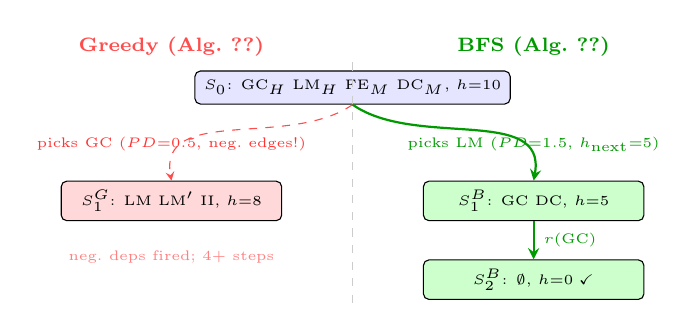
\begin{tikzpicture}[
  st/.style={draw, rectangle, rounded corners=2pt,
    minimum width=2.8cm, minimum height=0.42cm,
    text centered, font=\tiny},
  root/.style={st, fill=blue!10},
  good/.style={st, fill=green!20},
  bad/.style={st, fill=red!15},
  arr/.style={->, >=stealth, font=\tiny}]
  \node[root] (s0) at (0,0)
    {$S_0$: GC$_H$ LM$_H$ FE$_M$ DC$_M$,\ $h{=}10$};
  % Greedy branch
  \node[font=\tiny, red!80]   at (-2.3,-0.72) {picks GC\ ($PD{=}0.5$, neg.\ edges!)};
  \node[bad]  (s1g) at (-2.3,-1.44)
    {$S_1^G$: LM LM$'$ II,\ $h{=}8$};
  \node[font=\tiny, red!50]   at (-2.3,-2.15) {neg.\ deps fired; 4+ steps};
  % BFS branch
  \node[font=\tiny, green!60!black] at (2.3,-0.72) {picks LM\ ($PD{=}1.5$, $h_{\text{next}}{=}5$)};
  \node[good] (s1b) at (2.3,-1.44)
    {$S_1^B$: GC DC,\ $h{=}5$};
  \node[good] (s2b) at (2.3,-2.44)
    {$S_2^B$: $\emptyset$,\ $h{=}0$\;$\checkmark$};
  % Arrows
  \draw[arr, dashed, red!70]
    (s0.south) to[out=215,in=100] (s1g.north);
  \draw[arr, thick, green!60!black]
    (s0.south) to[out=325,in=80]  (s1b.north);
  \draw[arr, thick, green!60!black]
    (s1b) -- node[right]{\tiny $r(\mathrm{GC})$} (s2b);
  % Column labels
  \node[font=\scriptsize\bfseries, red!70]        at (-2.3,0.52) {Greedy (Alg.~\ref{alg:greedy})};
  \node[font=\scriptsize\bfseries, green!60!black] at ( 2.3,0.52) {BFS (Alg.~\ref{alg:bfs})};
  % Divider
  \draw[gray!40, dashed] (0,0.32) -- (0,-2.75);
\end{tikzpicture}
\caption{Greedy vs.\ BFS on $S_0{=}\{\text{GC}_H,\text{LM}_H,\text{FE}_M,\text{DC}_M\}$ ($w{=}0.5$).
Greedy may pick GC ($PD{=}0.5$), firing two ND edges ($h{:}10{\to}8$, 4+ steps).
BFS picks LM ($PD{=}1.5$, $h_{\text{next}}{=}5$); $h{:}10{\to}5{\to}0$, 2~steps, 0~new smells.}
\label{fig:bfs}
\end{figure}

\subsection{LLM-based refactoring agent}

Agent~I executes each step of the ordered plan within a LangGraph stateful
workflow.
For each smell in the ordered sequence, I: (i)~retrieves the source of the
affected class; (ii)~selects the refactoring technique from
Table~\ref{tab:smells}; (iii)~calls the LLM (GPT-4o or DeepSeek-Coder via
LiteLLM) with a chain-of-thought prompt specifying the smell type and
location; (iv)~validates the response against a Pydantic schema; and
(v)~writes the patched file to the repository.

Listing~\ref{lst:example} shows a representative Extract Method applied by Agent~I:
a 72-line \texttt{processOrder()} (SonarQube S138) is decomposed into three
single-responsibility helpers, reducing it to 18~LOC and eliminating a
co-occurring Feature Envy smell as a positive side effect.

\begin{lstlisting}[caption={Long Method (top) refactored by Agent~I via Extract Method (bottom).},label={lst:example}]
// BEFORE: processOrder() -- 72 LOC, S138 flagged
public void processOrder(Order o) {
  if (o == null || o.getItems().isEmpty())
    throw new IllegalArgumentException("Invalid order");
  // ... 23 more lines: discount rules, stock checks ...
  double total = 0;
  for (Item i : o.getItems())
    total += i.getPrice() * i.getQuantity();
  // ... 18 more lines: tax, currency conversion ...
  notificationService.send(o.getCustomer(), total);
  repository.save(o.withTotal(total));
  // ... 25 more lines: audit log, event publish ...
}

// AFTER: processOrder() -- 4 LOC, S138 resolved
public void processOrder(Order o) {
  validateOrder(o);                   // extracted
  double total = calculateTotal(o);   // extracted
  finalizeOrder(o, total);            // extracted
}

private void validateOrder(Order o) {
  if (o == null || o.getItems().isEmpty())
    throw new IllegalArgumentException("Invalid order");
  // ...
}
private double calculateTotal(Order o) {
  double total = 0;
  for (Item i : o.getItems())
    total += i.getPrice() * i.getQuantity();
  // ...
  return total;
}
private void finalizeOrder(Order o, double total) {
  notificationService.send(o.getCustomer(), total);
  repository.save(o.withTotal(total));
  // ...
}
\end{lstlisting}

%----------------------------------------------------------------------
\section{Experiment}
%----------------------------------------------------------------------

\subsection{Setup}

Planning agent decisions are evaluated against developer-committed refactoring
sequences from two datasets.
\textbf{RefactoringMiner~2.0}~\cite{tsantalis2022refactoringminer} provides
547 commits from 188 Java repositories with 15,562 annotated refactoring
instances (11,514 TP); key types used here are Extract Method (1,033~TP),
Move Method (266~TP), and Extract Class (108~TP).
\textbf{SWE-Refactor}~\cite{swerefactor2025} contributes 1,099 records from
18 projects (Guava, JUnit5, Checkstyle, Hibernate, and others) with 441
Extract Method and 410 Move Method instances.

For each evaluated commit we: (1) reconstruct the pre-refactoring smell set
$S_0$ from SonarQube; (2) run both agents to obtain two candidate first-step
actions; (3) compare each candidate against the refactoring type the developer
applied first.
A match is counted when the agent's selected smell type and refactoring
category agree with the developer's first committed operation.

In the \texttt{HttpJobExecutor} case (SWE-Refactor,
\texttt{shardingsphere-elasticjob}) both agents agree with the developer:
the Long Method (H, highest $PD$) is addressed first via Extract Method, which
also resolves Feature Envy (M) through a positive dependency, clearing both
smells in two steps with no negative effects.
This confirms that when no conflicting negative edges exist, the greedy score
correctly prioritises the highest-leverage smell.

%----------------------------------------------------------------------
\section{Discussion and Future Work}
%----------------------------------------------------------------------

We presented a multi-agent system in which the planning agent uses a formal
inter-smell dependency model to sequence refactoring operations before any
LLM agent modifies code.
The core claim is that the ordering problem cannot be solved by a greedy
heuristic when smells have active negative dependency edges, and that
state-space search with a total-severity heuristic avoids the traps that
cause greedy to introduce new smells.
The evaluated \texttt{HttpJobExecutor} case confirms that when no conflicting
negative edges are present the greedy score correctly prioritises the
highest-leverage smell---both agents agree with the developer's committed
sequence.
The LLM refactoring agent (I) demonstrates that individual operations---
once correctly ordered---can be executed with high structural fidelity, as
shown by the Extract Method example in Listing~\ref{lst:example}, which
eliminates both the Long Method and the co-occurring Feature Envy smell in
a single step via a positive dependency.

Several directions remain open for future work.
A labelled dataset of multi-smell Java classes---reconstructed from the
RefactoringMiner~2.0 and SWE-Refactor oracles---would enable comprehensive
evaluation of planning quality across hundreds of developer-committed
sequences, using metrics such as plan efficiency
$\eta = \text{steps}/\text{smells resolved}$, negative dependency rate
$\rho = \text{new smells introduced}/\text{refactorings executed}$, and
compile-and-test pass rate after each LLM-generated patch.

The dependency rules from Markovič~\&~Polášek~\cite{markovic2016refaktorovanie}
that underpin the planning agent could be validated against the empirical
smell-trajectory evidence of Cedrim et al.~\cite{cedrim2017}, whose
per-refactoring smell deltas would reveal which positive and negative
dependencies hold in practice and which require revision.

A scope-aware extension
$PD'_i = PD^{\mathrm{conc}}_i + \delta \cdot \mathrm{files\_affected}(s_i)$
would extend the current intra-class model to smells spanning multiple
compilation units, a case not yet handled by the dependency graph.

\section*{Acknowledgement}

This research and paper was 100\% funded by the EU NextGenerationEU through
the Recovery and Resilience Plan for Slovakia under the project
``InnovAIte Slovakia, Illuminating Pathways for AI-Driven Breakthroughs''
No.~09I02-03-V01-00029.

\begin{thebibliography}{00}

\bibitem{Fowler1999}
M.~Fowler,
\emph{Refactoring: Improving the Design of Existing Code}.
Boston, MA: Addison-Wesley, 1999.

\bibitem{chidamber1994metrics}
S.~R.~Chidamber and C.~F.~Kemerer,
``A metrics suite for object oriented design,''
\emph{IEEE Trans.\ Softw.\ Eng.},
vol.~20, no.~6, pp.~476--493, 1994.

\bibitem{lanza2006object}
M.~Lanza and R.~Marinescu,
\emph{Object-Oriented Metrics in Practice}.
Berlin: Springer, 2006.

\bibitem{fontana2016comparing}
F.~A.~Fontana, M.~V.~M{\"a}ntyl{\"a}, M.~Zanoni, and A.~Marino,
``Comparing and experimenting machine learning techniques for code smell
detection,''
\emph{Empir.\ Softw.\ Eng.}, vol.~21, no.~3, pp.~1143--1191, 2016.

\bibitem{yamashita2013exploring}
A.~Yamashita and L.~Moonen,
``Exploring the impact of inter-smell relations on software maintainability:
An empirical study,''
in \emph{Proc.\ ICSE}, San Francisco, CA, 2013, pp.~682--691.

\bibitem{palomba2018diffuseness}
F.~Palomba, G.~Bavota, M.~Di~Penta, F.~Fasano, R.~Oliveto,
and A.~De~Lucia,
``On the diffuseness and the impact on maintainability of code smells:
A large scale empirical investigation,''
\emph{Empir.\ Softw.\ Eng.}, vol.~23, no.~3, pp.~1188--1221, 2018.

\bibitem{abbes2011empirical}
M.~Abbes, F.~Khomh, Y.-G.~Gu{\'e}h{\'e}neuc, and G.~Antoniol,
``An empirical study of the impact of two antipatterns, blob and spaghetti
code, on program comprehension,''
in \emph{Proc.\ CSMR}, Oldenburg, Germany, 2011, pp.~181--190.

\bibitem{cedrim2017}
D.~Cedrim, A.~Garcia, M.~Mongiovi, R.~Gheyi, L.~Sousa,
R.~de~Mello, B.~Fonseca, M.~Ribeiro, and A.~Ch{\'a}vez,
``Understanding the impact of refactoring on smells: A longitudinal study
of 23 software projects,''
in \emph{Proc.\ ESEC/FSE}, Paderborn, Germany, 2017, pp.~465--475.

\bibitem{feng2020codebert}
Z.~Feng, D.~Guo, D.~Tang, N.~Duan, X.~Feng, M.~Gong, L.~Shou,
B.~Qin, T.~Liu, D.~Jiang, and M.~Zhou,
``CodeBERT: A pre-trained model for programming and natural languages,''
in \emph{Findings of EMNLP}, 2020, pp.~1536--1547.

\bibitem{10.1145/3691620.3695508}
D.~Wu, F.~Mu, L.~Shi, Z.~Guo, K.~Liu, W.~Zhuang, Y.~Zhong, and L.~Zhang,
``iSMELL: Assembling LLMs with expert toolsets for code smell detection
and refactoring,''
in \emph{Proc.\ ASE}, Sacramento, CA, 2024, pp.~1345--1357.

\bibitem{markovic2016refaktorovanie}
L.~Markovič and I.~Polášek,
``Refaktorovanie softvérových systémov,''
M.S.\ thesis, Dept.\ Applied Informatics,
Univ.\ of Ss.\ Cyril and Methodius, Trnava, Slovakia, 2016.

\bibitem{tsantalis2022refactoringminer}
N.~Tsantalis, A.~Ketkar, and D.~Dig,
``RefactoringMiner~2.0,''
\emph{IEEE Trans.\ Softw.\ Eng.}, vol.~48, no.~3, pp.~930--950, Mar.\ 2022.

\bibitem{swerefactor2025}
Y.~Xu, J.~Yang, and T.-H.~Chen,
``SWE-Refactor: A repository-level benchmark for real-world LLM-based
code refactoring,''
arXiv:2602.03712, Feb.\ 2026.

\bibitem{lenarduzzi2019}
V.~Lenarduzzi, N.~Saarim{\"a}ki, and D.~Taibi,
``The technical debt dataset,''
in \emph{Proc.\ PROMISE}, Porto de Galinhas, Brazil, 2019, pp.~2--11.

\bibitem{liang2025smelldetector}
W.~Liang, J.~Wang, H.-T.~Zheng, Y.~Li, H.~Lin, H.-G.~Kim,
B.~An, Z.~Wei, and Y.~Xu,
``SmellDetector: Multi-label code smell detection and refactoring with
large language models,''
in \emph{Proc.\ IJCNN}, 2025, pp.~1--8.

\end{thebibliography}

\end{document}
